\subsection{Red 'Tatooine-lan'}
Esta medición se trata de una red Wi-Fi doméstica de 4 dispositivos activos con un tiempo de escucha de 20 minutos. Dos de las máquinas estaban usando servicios de streaming de video.
\\

Mientras se realizaba la medición también se borraron los registros (comando 'arp -d $<host\_ip>$' en linux) la caché ARP en el dispositivo cuya IP pública es 190.168.0.14 y privada 192.168.0.12 con el objetivo de forzar un handshake en dicho protocolo con el default gateway de la red.
\\

Además, se reinició un dispositivo mientras se corría la escucha.

\subsubsection{Fuente S}
En la medición se contaron entre todos los paquetes del archivo \emph{.pcap} con la herramienta el ejercicio 1:

        \begin{itemize}
            \item 69834 paquetes unicast
            \item 289 paquetes broadcast (p.dst = 'ff:ff:ff:ff:ff')
            \item 70123 paquetes en total
        \end{itemize}

Dejando una entropía $H(S) = 0.03858550573957047$ y la siguiente distribución en la información de los símbolos $S_{broadcast}$ y $S_{unicast}$:

\begin{figure}[H]
	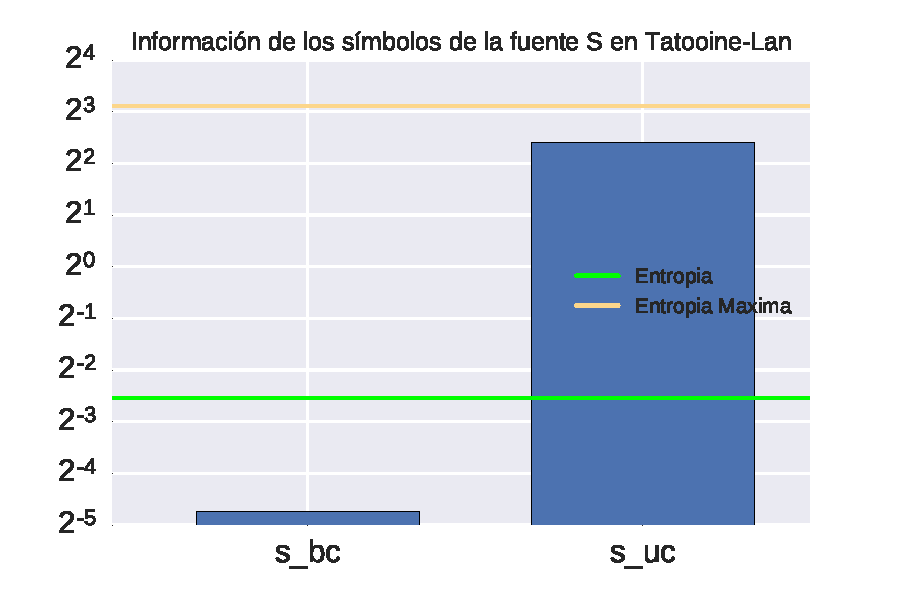
\includegraphics[width=15cm, height=12cm, keepaspectratio]{../img/barras-Tatooine-Lan.pdf}
\end{figure}

\newpage
\subsubsection{Grafo de conectividad de la red}
Con el fin de analizar de mejor manera la topología de la red también armamos un grafo entre los nodos de la red que muestre el tráfico de paquetes ARP sensado. Cada nodo está asociado a una IP y un eje entre una $IP_1$ y $IP_2$ significa que se sensó un paquete \emph{'who-has'} emitido por $IP_1$ consultando por la dirección MAC de $IP_2$.

\begin{figure}[H]
	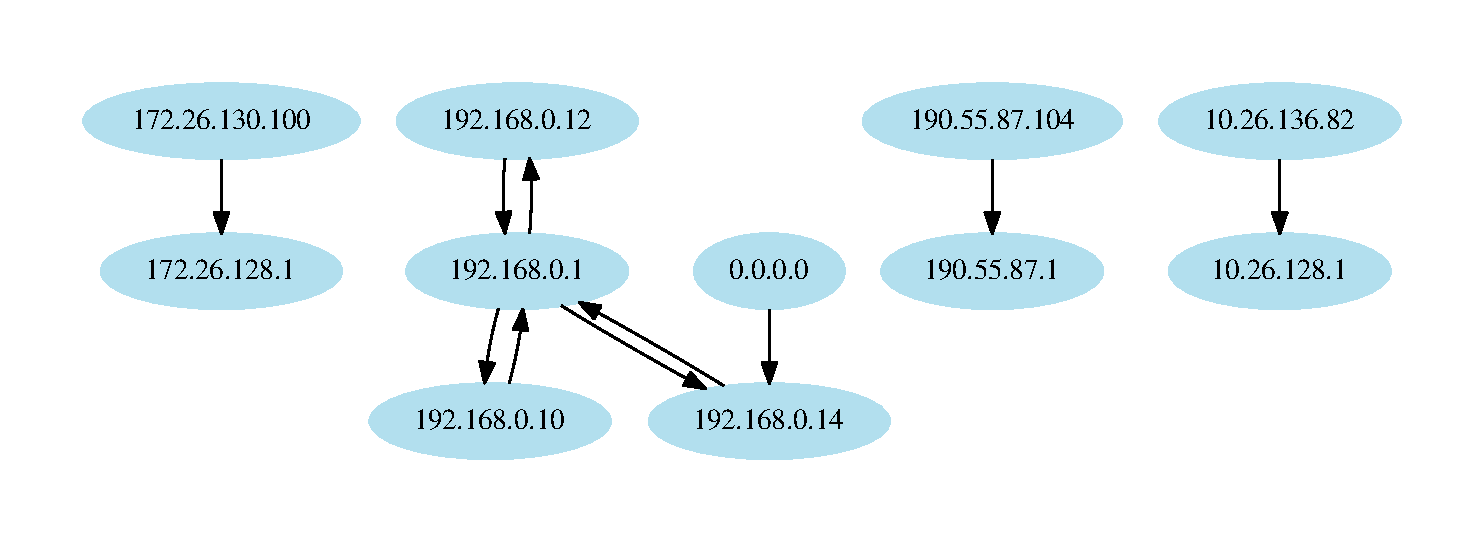
\includegraphics[width=15cm, height=8.7cm]{../img/red-Tatooine-Lan.pdf}
\end{figure}

Se puede notar que ninguno de los otros dispositivos mencionados, al margen de aquel para el cual flusheamos la caché ARP, hizo un request de tipo \emph{'who-has'} durante el sniff usando su IP pública. Dicho comportamiento se repite en las otras redes aledañas en las cuales un único nodo envía un paquete \emph{'who-has'} a una IP con el último octeto en 1 (candidatos a routers).
\\

Pero, por otro lado, se puede ver buena actividad en una red que parece corresponderse con el rango 192.168.0.0/16 reservado para IPs privadas. Como la capa de enlace se encarga de que las redes privadas no se solapen, podemos afirmar que se trata de la red a la que nos conectamos durante la medición.
\\

Es interesante la aparición de una IP 0.0.0.0, la cual se asigna a dispositivos en diferentes situaciones. Entre ellos, cuando un dispositivo se inicializa en una red y envía su primer paquete DHCP (sin conocer todavía su IP en la red). Por lo tanto, tiene sentido que dicha interacción se deba al dispositivo reiniciado mencionado antes.

\subsubsection{Información y nodos distinguidos}
Haciendo uso de la herramienta del ejercicio 2 para distinguir nodos de la red respecto de sus respectivos símbolos en la fuente $S_1$ en caso de que aporten menor información que la entropía de dicha fuente, encontramos únicamente al nodo 192.168.0.1 como nodo distinguido.
\\

Las direcciones con los dos últimos octetos en 0.1 en redes 192.168.0.0/16 son comunes para IPs de interfaces de routers. Lo que significaría que nuestro código fue capaz de encontrar al menos un default gateway, particularmente por el que más nodos consultaron.

\begin{figure}[H]
	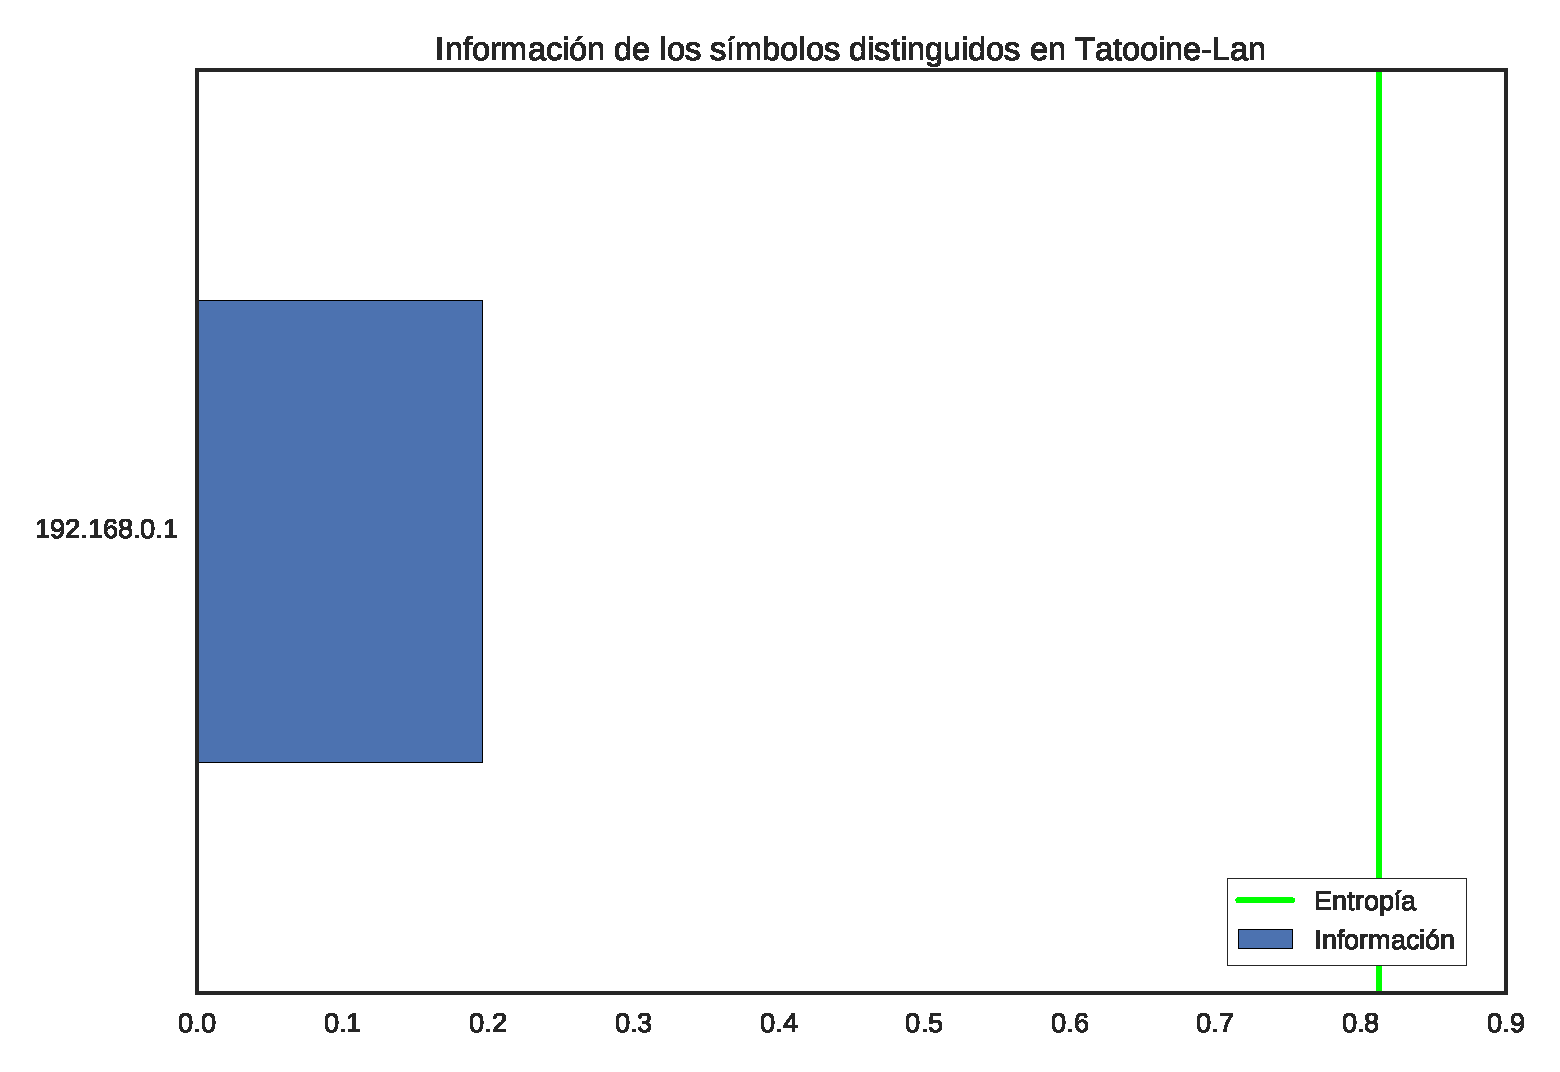
\includegraphics[width=15cm, height=8cm]{../img/distinguidos-Tatooine-Lan.pdf}
\end{figure}
